% =====================================================================
% VERSION ENSAE, REDUCTION SFE (phase 3, 1er octobre 2026) : chapitre 3, donnees.
% Copie a texte constant de chapitres/05_donnees_limites.tex.
% Ne changent que les titres et les renvois repares, listes dans
% reduction/phase3.md.
% Lu par main_ensae.tex seul : ne jamais le faire lire par main_institut.tex,
% qui garde chapitres/.
% =====================================================================

\chapter{Données}
\label{chap:donnees}
\label{part:donnees}

% MIGRÉ AUTOMATIQUEMENT depuis memoire/main.tex (plages 1002-1433).
% Hiérarchie descendue d'un cran, labels préfixés "don:".
% RELECTURE FAITE (août 2026). Aucune phrase du chapitre n'annonce la copule ni
% la variable latente comme LE modèle. Ajouts d'août : la table des trois
% fréquences, le seuil de collecte, et la section des deux biais chiffrés
% (élasticité de taille corrigée par troncature, chain-ladder de remontée).
%==============================================================

Quelles entrées du calcul les données permettent-elles d'estimer ? Nous séparons les montants
de pertes, les nombres d'incidents et les parts des vecteurs d'attaque. Le tableau suivant attribue
à chaque source son rôle. Les états de conformité et les transmissions entre piliers ne sont
observés dans aucune de ces bases : ils resteront des hypothèses du calcul.

%--------------------------------------------------------------
%--------------------------------------------------------------
\section{Sources et rôles}
\label{sec:carto}
%--------------------------------------------------------------

\begin{center}
\renewcommand{\arraystretch}{1.3}
\begin{tabular}{>{\raggedright}p{2.75cm} >{\raggedright}p{2.6cm} >{\raggedright}p{3.9cm} >{\raggedright\arraybackslash}p{4.05cm}}
\toprule
\rowcolor{lightblue}
\textbf{Source} & \textbf{Effectif retenu} & \textbf{Rôle dans le modèle} & \textbf{Justification / limite} \\
\midrule
PRC 2025 & $15\,053$ incidents, 2019 à 2025 & Sévérité alternative via conversion Jacobs ; nombre annuel de notifications $\lambda_{ref}$, décrit et non utilisé par le moteur &
Périmètre défini, mais sévérité dérivée d'un modèle log-log \\
\addlinespace
SAS OpRisk Global & $41\,975$ pertes, dont $570$ en cyber $\times$ finance de 2000 à 2026 & Sévérité (montants réels) et nombre annuel d'incidents du moteur ($\lambda$) &
Montants observés, mais biais vers les grandes entités financières \\
\addlinespace
Hackmageddon & $1\,041$ incidents, premier semestre 2026 & Parts par vecteur d'attaque (structure du risque) &
Ne fixe aucun niveau : pondère le multiplicateur qui fait passer $\lambda$ d'un état de conformité à l'autre \\
\bottomrule
\end{tabular}
\end{center}

Les articles~19 et~231 du règlement délégué (UE) 2015/35 exigent des données exactes, exhaustives et
appropriées, pour les provisions techniques et pour un modèle interne ; nous prenons ces critères pour référence. Aucune des bases que nous avons examinées ne remplit ces trois exigences. Nous documentons les biais de chaque source et leurs retraitements.

% SOURCES-SCRIPTS: 63 104

\section{Biais statistiques des sources}
\label{sec:trois-biais}

Trois biais affectent les bases PRC et OpRisk. Le
\emph{biais de sélection} touche OpRisk, qui recense surtout des pertes rendues publiques, donc
celles des grandes entités ou des montants exceptionnels. Il surreprésente les événements extrêmes.
Nous adaptons les pertes à la taille par une élasticité de sévérité, variation relative de la perte associée à une variation relative de taille, estimée
(\S\ref{sec:biais-chiffres}).

Pour la fréquence, le \S\ref{sec:ancrage} distingue l'exposant estimé
sur tout le registre et celui, retenu, des grandes institutions. Le \emph{biais de déclaration}
touche la PRC, car la notification des fuites de données personnelles est obligatoire dans la plupart
des États américains, pas celle d'un rançongiciel qui n'exfiltre rien. Le niveau de fréquence est
donc lu sur OpRisk, et la répartition par vecteur sur Hackmageddon.

Un \emph{biais de survie} pourrait sous-représenter les entités disparues, mais les pertes qui ont conduit à une faillite sont souvent publiques. Ces bases n'en donnent ni l'existence ni le signe, et il ne figure pas parmi les écarts mesurés du chapitre~\ref{ch:robustesse}.

\section{Hétérogénéité temporelle et actualisation des sinistres}

Le sous-échantillon cyber-finance OpRisk contient des pertes de $1979$ à $2026$, période sur laquelle les montants nominaux dérivent.
Pour chaque perte, la base donne le montant de l'année de l'événement et sa valeur courante, corrigée
de l'inflation générale. Leur rapport, égal à un pour les années récentes, atteint $1{,}747$ en
$2004$, d'où une inflation implicite de $2{,}19\,\%$ par an. Nous calibrons cependant sur le premier,
c'est-à-dire sur des montants \emph{nominaux}. Ce choix minore les sinistres anciens ramenés en euros
courants, donc la queue et le capital. Son effet sur la dérive des pertes est mesuré au
\S\ref{soc:sec:backtest}.
% SOURCES-SCRIPTS: 102

La PRC fournit la fréquence de référence $\lambda_{ref}$, qui compte des notifications sans seuil de
matérialité et ne fixe pas le niveau du capital. Elle sert aussi de source de sévérité indirecte : la conversion de \citet{jacobs2014}, $\ln(L) = 7{,}68 + 0{,}76\,\ln(X)$, donne la perte $L$ en dollars d'un incident à partir de son nombre $X$ d'enregistrements. Calibrée sur les $15\,053$ incidents 2019--2025 dont le volume touché est renseigné (la figure~\ref{fig:composition-temporelle-rapport} compte toutes les notifications), la queue PRC a un paramètre de forme $\hat{\xi}_{\text{PRC}} = 1{,}03$ (intervalle à $90\,\%$ :
$[0{,}97~;~1{,}09]$). À cette valeur, l'espérance est infinie. On ne la lit qu'avec le plafond de sévérité
propre à cette source \matcomp.

\begin{figure}[H]
\centering
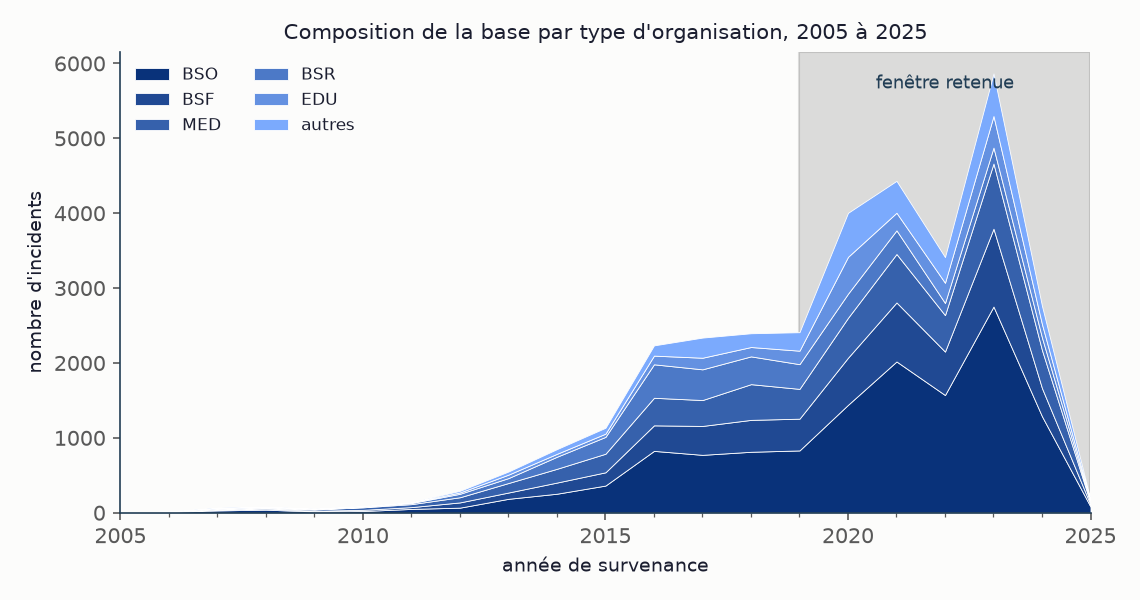
\includegraphics[width=0.78\textwidth]{D4_composition_temporelle.png}
\caption{Composition de la chronologie PRC par type d'organisation et par année. La zone grisée est
la fenêtre retenue. La hausse d'avant $2019$ suit l'extension de la collecte. La baisse de $2025$ traduit le manque de recul. BSF : organisations financières ; les autres codes sont ceux de la base.}
% SOURCES-SCRIPTS: 104
\label{fig:composition-temporelle-rapport}
\end{figure}



% SOURCES-SCRIPTS: 57 62 63

\section{Fréquences et seuils de collecte}

% SOURCES-SCRIPTS: 08b 60 62 136

La valeur de la fréquence dépend du périmètre de comptage de la source. Sur le
panel firme-année du SAS OpRisk (sous-catégories TIC, 2005--2022), le taux est de $0{,}10$ événement
par firme et par an toutes firmes confondues, et $0{,}21$ pour les firmes à au moins dix événements.

Au chapitre~\ref{chap:resultats}, nous estimons $\lambda$ comme une fonction de la taille de firme afin
de le lire à celle de l'entité notionnelle, ce qui donne $0{,}021$ avec l'exposant estimé sur les grandes institutions. Ces taux sont par firme ; celui du moteur compte le périmètre financier étudié. Le panel d'entité retient cinq sous-catégories TIC, plus larges que le filtre cyber-finance de sévérité : leur réconciliation reste nécessaire. Tous ne retiennent que les pertes au-dessus du seuil de collecte d'OpRisk. Ils comptent
donc les incidents TIC \emph{matériels}, pas tous les incidents au sens du reporting DORA.

Le taux par firme est une propriété d'entité, lisible sur un panel. Le tableau~\ref{tab:echelle} traduit ces échelles en capital.

Le terme de fréquence recouvre trois taux, à trois niveaux d'observation :
\begin{center}\small
\renewcommand{\arraystretch}{1.3}
\begin{tabular}{@{}l l r p{5.1cm}@{}}
\toprule
\textbf{Symbole} & \textbf{Source} & \textbf{Valeur} & \textbf{Ce qu'il compte} \\
\midrule
$\lambda_{ref}$ & PRC & $341$/an & notifications de violation de données des
\emph{organisations financières} de la base PRC (code \texttt{BSF}), et non de la base
entière, qui en compte $2\,150$ par an. Décomposée par vecteur d'attaque ; n'entre pas dans le moteur et ne fixe aucun niveau de capital. \\
$\lambda$ & OpRisk & $21{,}6$/an & incidents TIC \emph{matériels} du
périmètre financier étudié. C'est l'entrée du moteur pour les capitaux de ce périmètre. \\
$\lambda_{\text{entité}}$ & OpRisk & $0{,}021$/an & les événements TIC du panel, rapportés
à \emph{une} firme et lus \emph{à la taille} de l'entité notionnelle. C'est
l'échelle de lecture d'une entité soumise à DORA. \\
\bottomrule
\end{tabular}
\end{center}
Le facteur $16\,307$ entre $\lambda_{ref}$ et $\lambda_{\text{entité}}$ sépare trois comptages, ceux des notifications, des pertes
matérielles du secteur et des pertes matérielles par entité. Les capitaux du périmètre financier
reposent sur $\lambda$ ; les besoins d'entité utilisent la fréquence $\lambda(A)$ du panel
(\S\ref{sec:ancrage}).
% SOURCES-SCRIPTS: 67 136

\section{Effet chiffré de deux biais}
\label{sec:biais-chiffres}
% SOURCES-SCRIPTS: 57

Corrigée de la troncature au seuil de collecte, l'élasticité de la sévérité à la taille est de
$b=0{,}087$, et la sévérité transposée à l'entité notionnelle n'est multipliée que par $0{,}861$. Le
biais de taille est mesuré dans le registre. Sous les hypothèses du chain-ladder, les $97$ événements observés sur 2023--2025 deviennent $255$ à l'ultime, soit $85{,}0$ par an contre $74{,}1$ sur 2015--2022, et la fréquence est relevée d'un facteur $1{,}147$. Cette projection suggère un retard de
remontée, sans établir l'évolution du risque TIC réel. Les régressions et le triangle de
développement sont déportés \matcomp.
% SOURCES-SCRIPTS: 67

Les deux corrections se compensent presque sur la perte moyenne, $0{,}861\times1{,}147=0{,}987$, soit
un effet net de $1{,}3\,\%$, inférieur à l'incertitude d'estimation de chacune, mais elles ne se compensent pas sur le capital. À queue lourde, le quantile à $99{,}5\,\%$ répond à la sévérité bien plus qu'à la fréquence. Leur effet net sur le capital n'est pas chiffré. La correction de taille agit sur la sévérité et celle de troncature sur la fréquence ; leur compensation sur la moyenne ne détermine pas le signe de l'effet sur le quantile.

\section{Hackmageddon et la structure du risque}
\label{sec:hackmageddon}

Hackmageddon donne la \emph{structure} du risque, jamais son niveau. Le décompte retenu couvre le
semestre janvier--juin 2026, avec 1\,041 incidents, dont 840 à vecteur d'accès initial identifié
($81\,\%$). Le jeu consulté n'a pas été conservé ; relu en octobre 2026 avec une autre grille, il ne redonne pas ces décomptes à l'unité. Ce sont des citations datées. Ils fixent les parts de répartition par vecteur, qui pondèrent le
multiplicateur de fréquence entre états de conformité (\S\ref{sec:quatre-canaux}). Ce
multiplicateur hérite donc de leur statut de citation.

\begin{center}
\renewcommand{\arraystretch}{1.3}
\begin{tabular}{>{\raggedright}p{5cm} c >{\raggedright\arraybackslash}p{6cm}}
\toprule
\rowcolor{lightblue}
\textbf{Vecteur d'attaque} & \textbf{Part} & \textbf{Exigence DORA} \\
\midrule
Hameçonnage / ingénierie sociale & $38{,}8\,\%$ & Art.~13, sensibilisation \& formation \\
Exploitation vuln.\ exposée & $33{,}8\,\%$ & Art.~26, tests TLPT ; Art.~8--10 \\
Chaîne d'approvisionnement / tiers TIC & $15{,}8\,\%$ & Art.~28--44, gestion du risque tiers \\
Identifiants compromis & $6{,}3\,\%$ & Art.~9, contrôle d'accès \& MFA \\
\bottomrule
\end{tabular}
\end{center}

Deux parts structurent les scénarios du chapitre~\ref{chap:multietats} : $15{,}8\,\%$ des attaques
empruntent le vecteur tiers, objet des articles~28 à~44, et $49{,}6\,\%$ (dont ces $15{,}8\,\%$) relèvent de vecteurs qu'un
test TLPT est censé détecter en amont. La base recense des incidents rendus publics, ce qui interdit
d'en tirer un niveau de fréquence, et sa taxonomie est instable. La catégorie rançongiciel n'existait
pas en 2023, et une lecture naïve lui prête une hausse de 11 points là où, après reclassement, elle recule de 23 points. Seules les motivations se comparent directement dans le temps. Les catégories bâloises de la base SAS informent trop faiblement la sévérité pour fonder une segmentation (\S\ref{sec:profilage-variables}).

% SOURCES-SCRIPTS: 63

\section{OpRisk Global et la sévérité en euros}
\label{sec:oprisk}

% SOURCES-SCRIPTS: 07 47 63

OpRisk Global est la base de référence historique du risque opérationnel au sens de Bâle. Le risque cyber y est reconstruit à
partir des catégories \og Systems Security\fg{} et \og Business Disruption and System Failures\fg{}, et
le périmètre cyber $\times$ finance retient $570$ pertes de 2000 à 2026, soit $27$ années. La base courante en compte douze de plus, antérieures à 2000. La fréquence gelée, $582/27 = 21{,}56$ incidents par an, les compte, alors que l'échantillon de sévérité n'en compte que $570$ ($570/27 = 21{,}11$). Elle dépasse ainsi de $2{,}1\,\%$ celle de l'échantillon. Le dénominateur de $27$ ans compte l'année 2026, incomplète à la date de l'extraction (cinq pertes), si bien que le sens de l'écart sur le niveau de fréquence n'est pas établi ; nous le déclarons sans corriger la valeur (\S\ref{sec:pu-coherence}). \citet{elingwirfs2019}
en extraient également les pertes d'origine informatique. Cette base alimentait les modèles internes de
mesure avancée (section~\ref{chap:reglementaire}), qui calibraient la sévérité extrême sur des pertes
observées sans passer par un indicateur de volume. Nous reprenons cette logique.

Sur la population de la fréquence (secteur financier, catégories TIC, 2005--2022, $1\,476$
observations), la sévérité se décrit ainsi :
\begin{center}
\renewcommand{\arraystretch}{1.3}
\begin{tabular}{l r l r}
\toprule
\rowcolor{lightblue}
\textbf{Indicateur} & \textbf{Valeur} & \textbf{Indicateur} & \textbf{Valeur} \\
\midrule
Médiane & 1{,}20 M\$ & P99 & 419{,}3 M\$ \\
Moyenne & 33{,}8 M\$ & Maximum & 10\,970{,}8 M\$ \\
P90 & 25{,}3 M\$ & Total cumulé & 49{,}8 Md\$ \\
\bottomrule
\end{tabular}
\end{center}
Les montants de ce tableau sont en dollars ; le moteur les convertit en euros au taux fixe de $0{,}92$. Le décile supérieur concentre $92{,}3\,\%$ de la perte totale et le centile supérieur $65{,}1\,\%$,
ce qui justifie la théorie des valeurs extrêmes du chapitre~\ref{chap:socle}.
% SOURCES-SCRIPTS: 67

Nous ajustons la loi de Pareto généralisée sur les $570$ pertes cyber $\times$ finance au-delà d'un
seuil $u = 20$~M\euro, qui est le percentile~85 des montants et où le graphique des excès moyens devient
linéaire (figure au supplément, \S\ref{don:fig:mep}). Avec $86$ excès, soit un taux de dépassement de $86/570 = 0{,}1509$, on obtient :
\[
\hat{\xi} = 0{,}595 \quad (\text{IC}_{90\%}=[0{,}30\,;\,0{,}83]), \qquad
\hat{\sigma} = 58{,}0~\text{M\euro}, \qquad
\qsev_{99{,}5\%}(X) = 663~\text{M\euro}.
\]
Le dernier terme est le quantile de la sévérité d'un sinistre, pas un capital, car le besoin de capital
est le quantile de la charge annuelle agrégée, obtenu par composition avec la fréquence. L'intervalle
bootstrap de ce quantile, $[411\,;\,1037]$~M\euro, couvre un facteur~2{,}5. L'écart avec la PRC
($\hat{\xi}_{\text{PRC}} = 1{,}03$) ne mesure pas une différence de risque : la sévérité PRC
est une puissance de pente $0{,}76$ du nombre d'enregistrements, et une puissance multiplie l'indice
de queue par son exposant. Les deux indices sont positifs ($\xi > 0$), sur deux objets différents.

%--------------------------------------------------------------
\section{Analyse exploratoire et profilage des variables}
\label{sec:profilage-variables}
%--------------------------------------------------------------
% SOURCES-SCRIPTS: 104

Les variables disponibles ne permettent pas de segmenter la sévérité, ce qui justifie la queue
commune ajustée ci-dessus. Le profilage, détaillé dans le supplément, montre d'abord que, dans la
chronologie PRC, un champ non renseigné prend la valeur \texttt{UNKN} au lieu d'être vide. Le nombre d'enregistrements touchés n'est ainsi documenté que dans $41{,}77\,\%$ des cas. De plus, la base n'agrège pas les
notifications, si bien qu'un même incident déclaré à plusieurs autorités y figure plusieurs fois. La
déduplication retire $1\,643$ lignes, soit $10{,}9\,\%$ des lignes, une borne basse. Nous n'additionnons jamais ces volumes, mais les doublons pèsent encore sur les comptages et sur l'ajustement de la sévérité ; leur effet n'est pas chiffré.

La chronologie PRC compte $74\,783$ incidents, dont $31\,217$ documentent un volume touché
positif. La base SAS compte $41\,976$ lignes brutes et $41\,975$ pertes après retrait d'une
aberration de saisie, dont $1\,099$ en catégories TIC et $570$ dans le croisement cyber $\times$
finance retenu pour la sévérité. Le tableau donne pour chaque variable son type, son rôle et la part
de lignes renseignées, \texttt{UNKN} compté comme un manquant.

\begin{center}\footnotesize
\renewcommand{\arraystretch}{1.05}
\begin{tabular}{@{}>{\ttfamily\raggedright}p{3.35cm} l >{\raggedright}p{5.1cm} l r@{}}
\toprule
\textbf{Variable} & \textbf{Type} & \textbf{Rôle dans le modèle} & \textbf{Base} & \textbf{Renseignée} \\
\midrule
total\_affected & quantitative & enregistrements touchés, seule mesure d'impact de la base & PRC & $41{,}77\,\%$ \\
residents\_affected & quantitative & sous-ensemble territorialisé du précédent & PRC & $79{,}88\,\%$ \\
breach\_date & temporelle & date de survenance, support de la fréquence annuelle & PRC & $54{,}82\,\%$ \\
reported\_date & temporelle & date de notification, support du délai de détection & PRC & $99{,}54\,\%$ \\
end\_breach\_date & temporelle & fin d'exposition, support de la durée d'incident & PRC & $28{,}18\,\%$ \\
organization\_type & qualitative & classe d'organisation, huit modalités & PRC & $89{,}29\,\%$ \\
breach\_type & qualitative & vecteur de la brèche, huit modalités & PRC & $47{,}31\,\%$ \\
\midrule
Loss Amount & quantitative & montant de perte avérée, source de la sévérité & SAS & $100\,\%$ \\
Event Risk Category & qualitative & catégorie bâloise de niveau 1, sept modalités & SAS & $100\,\%$ \\
Sub Risk Category & qualitative & sous-catégorie, définit le périmètre TIC & SAS & $100\,\%$ \\
Basel Business Line & qualitative & ligne métier, dix modalités & SAS & $100\,\%$ \\
Industry Sector Name & qualitative & secteur, définit le périmètre financier & SAS & $100\,\%$ \\
Revenue & quantitative & chiffre d'affaires, mesure de taille & SAS & $87{,}82\,\%$ \\
Assets & quantitative & actif total, mesure de taille prudentielle & SAS & $83{,}51\,\%$ \\
\bottomrule
\end{tabular}
\end{center}

Le volume touché est la variable d'impact la moins bien renseignée, et ce n'est pas un hasard de collecte. Les champs qu'impose l'obligation de notification, la date de déclaration et la nature de l'organisation, sont remplis. Ceux qui demandent une enquête, le volume touché et la date réelle de survenance, ne le sont pas. Ce profil est compatible avec des difficultés d'enquête ; son lien à la gravité reste à établir. Il ne se confond pas avec le biais de déclaration de la section~\ref{sec:trois-biais}, qui joue sur les incidents entrant dans la base, alors que le manquant joue sur les champs remplis au sein d'incidents déjà entrés. Le signe de leur effet conjoint n'est pas établi. Seul le second se décrit sur les champs observés.

\begin{figure}[H]
\centering
\begin{subfigure}{0.49\textwidth}
  \centering
  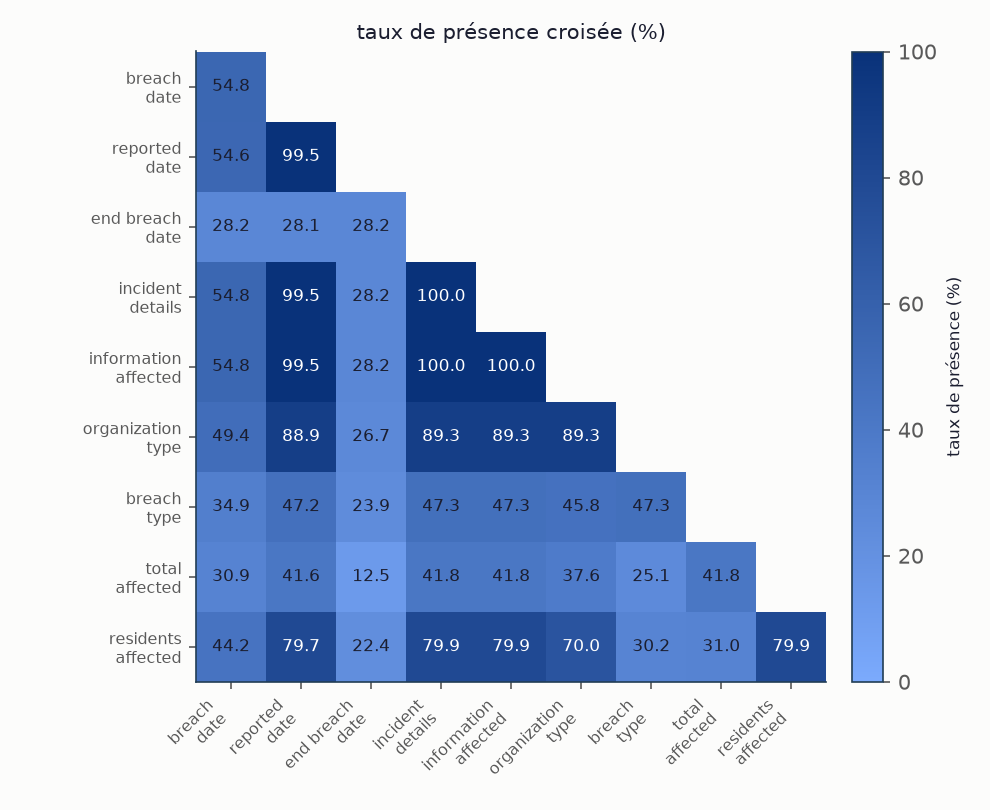
\includegraphics[width=\linewidth]{D1a_presence_taux.png}
  \caption{}\label{fig:presence-taux}
\end{subfigure}\hfill
\begin{subfigure}{0.49\textwidth}
  \centering
  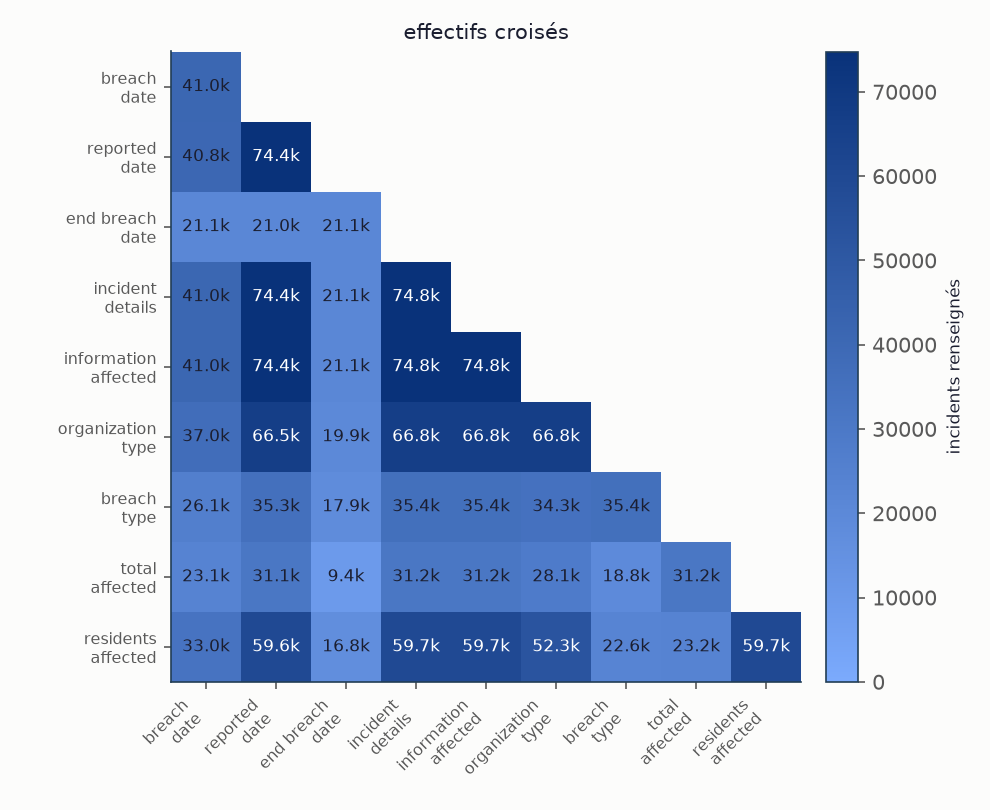
\includegraphics[width=\linewidth]{D1b_presence_effectifs.png}
  \caption{}\label{fig:presence-effectifs}
\end{subfigure}
\caption{Présence croisée des variables de la chronologie PRC, en taux (a) et en effectifs (b). Le
volume touché n'est renseigné en même temps que le type de brèche que dans $25{,}1\,\%$ des cas, et en
même temps que la date de fin d'exposition que dans $12{,}5\,\%$ des cas.}
% SOURCES-SCRIPTS: 104
\label{fig:presence-croisee}
\end{figure}

Les $12{,}5\,\%$ du croisement le plus pauvre représentent encore plus de neuf mille incidents. La
matrice montre surtout que les lacunes se cumulent. Une analyse qui croiserait le volume touché, le type de brèche et la durée
d'exposition ne disposerait plus que de $10{,}9\,\%$ de la base. Rien n'indique que cette fraction
soit représentative, puisque les trois manques ont la même origine. Le modèle ne
conditionne donc la sévérité sur aucune de ces variables.

\subsection{Variables d'impact}
\label{subsec:describe-impact}

Nous publions des quantiles de sévérité dans plusieurs chapitres. Le tableau suivant les réunit pour
les quatre variables d'impact, de sorte qu'on puisse juger la queue avant de lire l'ajustement.

\begin{center}\small
\renewcommand{\arraystretch}{1.1}
\begin{tabular}{@{}l r r r r@{}}
\toprule
& \multicolumn{2}{c}{\textbf{PRC}} & \multicolumn{2}{c}{\textbf{SAS OpRisk}} \\
\cmidrule(lr){2-3}\cmidrule(lr){4-5}
& \textbf{enregistrements} & \textbf{sévérité dérivée} & \textbf{toutes catég.} &
\textbf{cyber $\times$ finance} \\
& (nombre) & (M\euro) & (M\euro) & (M\euro) \\
\midrule
$n$              & $15\,053$     & $15\,053$   & $41\,975$  & $570$ \\
moyenne          & $102\,646$    & $6{,}07$    & $69{,}98$  & $24{,}18$ \\
écart-type       & $1\,235\,098$ & $41{,}59$   & $647{,}26$ & $98{,}50$ \\
minimum          & $1$           & $0{,}0020$  & $0{,}0920$ & $0{,}0920$ \\
\midrule
$q_{25}$         & $69$          & $0{,}0497$  & $1{,}012$  & $0{,}343$ \\
médiane          & $1\,104$      & $0{,}409$   & $3{,}763$  & $1{,}380$ \\
$q_{75}$         & $8\,330$      & $1{,}901$   & $18{,}40$  & $8{,}211$ \\
$q_{85}$         & $23\,467$     & $4{,}176$   & $45{,}40$  & $20{,}03$ \\
$q_{90}$         & $49\,000$     & $7{,}307$   & $82{,}90$  & $45{,}47$ \\
$q_{95}$         & $164\,673$    & $18{,}36$   & $202{,}4$  & $102{,}1$ \\
$q_{99}$         & $1\,719\,753$ & $109{,}2$   & $1\,012$   & $377{,}8$ \\
maximum          & $60\,000\,000$& $1\,624$    & $53\,360$  & $1\,380$ \\
\midrule
$q_{99}/$médiane & $1\,558$      & $267$       & $269$      & $274$ \\
maximum$/q_{99}$ & $34{,}9$      & $14{,}9$    & $52{,}7$   & $3{,}7$ \\
coef. de variation & $12{,}03$   & $6{,}85$    & $9{,}25$   & $4{,}07$ \\
\bottomrule
\end{tabular}
\end{center}
% SOURCES-SCRIPTS: 104

\vspace{2pt}
\noindent La première colonne compte des enregistrements, les trois autres des euros, et elles
ne se comparent ni en niveau ni en quantile. La quatrième porte la calibration publiée. Sur les quatre
colonnes, la moyenne dépasse le troisième quartile : une distribution dans ce cas ne se décrit pas par
sa moyenne, parce qu'une minorité d'observations en fait le niveau. Le rapport du $q_{99}$ à la médiane
est voisin de $270$ sur les trois colonnes monétaires et monte à $1\,558$ sur les enregistrements. La
queue ne se prolonge pas, elle change d'échelle. Le coefficient de variation atteint $4{,}07$ sur le
périmètre calibré et jusqu'à $12{,}03$ sur les enregistrements, alors qu'il vaut exactement un pour une
loi exponentielle.

Un détail évite un contresens. Le rapport du maximum au $q_{99}$ vaut $3{,}7$ sur le périmètre cyber
$\times$ finance, contre $52{,}7$ sur la base entière. Le périmètre retenu est donc le moins extrême
des deux, car le sinistre le plus lourd du fichier ne relève pas du risque informatique. Ce sinistre
n'entre donc pas dans le périmètre calibré ; la dépendance de la queue calibrée à ses plus grosses
pertes est mesurée au chapitre~\ref{chap:socle}.

\subsection{Plus gros incidents et concentration}
\label{subsec:top-incidents}

Une queue lourde reste abstraite tant qu'on ne voit pas les événements qui la forment. Le tableau
liste les plus gros incidents de la chronologie PRC, comptés en enregistrements. Il illustre la forme de
la queue, mais pas le quantile publié, qui est calibré en euros sur OpRisk.

\begin{center}\footnotesize
\renewcommand{\arraystretch}{1.08}
\begin{tabular}{@{}l l l r@{}}
\toprule
\textbf{Organisation} & \textbf{Secteur} & \textbf{Survenance} &
\textbf{Enregistrements} \\
\midrule
Progress Software, Ipswitch, Inc.     & services & 2023-05-27 & $60\,000\,000$ \\
T-Mobile USA, Inc.                    & services & 2021-08-13 & $53\,700\,000$ \\
AT\&T Inc.                            & services & 2024-03-26 & $51\,226\,382$ \\
Logan Health Medical Center           & santé    & 2021-11-22 & $40\,000\,000$ \\
T-Mobile                              & services & 2022-11-25 & $37\,000\,000$ \\
Comcast Cable Communications LLC      & services & 2023-10-16 & $35\,879\,455$ \\
Zoosk, Inc.                           & services & 2020-01-12 & $24\,200\,000$ \\
CafePress, Inc.                       & détail   & 2019-02-19 & $23\,000\,000$ \\
Texas Dow Employees Credit Union      & finance  & 2023-05-29 & $20\,000\,000$ \\
Evite, Inc.                           & services & 2019-02-22 & $18\,571\,486$ \\
loanDepot.com, LLC                    & finance  & 2024-01-03 & $16\,924\,071$ \\
ClearVoiceResearch.com, LLC           & services & 2021-04-16 & $15\,700\,000$ \\
\bottomrule
\end{tabular}
\end{center}
% SOURCES-SCRIPTS: 104

\vspace{2pt}
\noindent Le premier incident est la compromission du logiciel de transfert de fichiers évoquée au
chapitre~\ref{chap:cadre-cyber-dora} comme choc de cause commune. La base le range sous le nom de
l'éditeur, et non sous celui des milliers d'organisations atteintes à travers lui. Deux entrées
distinctes concernent le même opérateur de télécommunications, à quinze mois d'intervalle. Les deux
incidents financiers, un établissement de crédit et un prêteur hypothécaire, dépassent chacun quinze
millions d'enregistrements.

La moitié du volume de sept années tient dans $31$ incidents sur $13\,410$, soit $0{,}23\,\%$ de la
base. Quatre-vingts pour cent tiennent dans $209$ incidents, et quatre-vingt-dix pour cent dans $491$.
Un modèle qui décrirait cette distribution par son centre manquerait son objet, puisque le niveau vient
d'une poignée d'événements et non du régime courant. L'ajustement par dépassement de seuil formalise
cette idée, et c'est aussi pourquoi le quantile qui fonde le besoin de capital est atteint par un
sinistre unique plutôt que par une accumulation.

Des doublons de notification restent visibles dans le tableau. La déduplication du début de section
exige une égalité exacte sur l'organisation, le volume et la date ; elle ne rapproche ni deux graphies
d'une même raison sociale ni deux notifications décalées d'un jour.

Avant $2015$, la
chronologie ne porte que $2\,152$ incidents, soit $6{,}5\,\%$ de la période $2005$--$2025$. Le maximum
est atteint en $2023$ avec $5\,866$ incidents, et l'exercice $2025$ n'en compte que $174$, soit
$3{,}0\,\%$ du pic, faute de notifications déjà enregistrées (figure~\ref{fig:composition-temporelle-rapport}).
Ces deux déformations vont en sens contraire, et aucune ne signale un risque. Une fenêtre plus large
fabriquerait un régime calme au début et un effondrement à la fin, et un modèle de tendance ajusté
dessus mesurerait la maturation d'une base de données. Nous nous en tenons donc à la fenêtre grisée,
comme pour la validation hors échantillon.

Compter les incidents et sommer les volumes ne classent pas les catégories dans le même ordre. La
figure~\ref{fig:organisation-double-axe} met en regard le nombre d'incidents et le volume touché par type
d'organisation. Les deux ordres divergent sur quatre types sur sept. Le commerce de détail est sixième en
nombre et quatrième en volume, l'enseignement quatrième en nombre et cinquième en volume.

\begin{figure}[H]
\centering
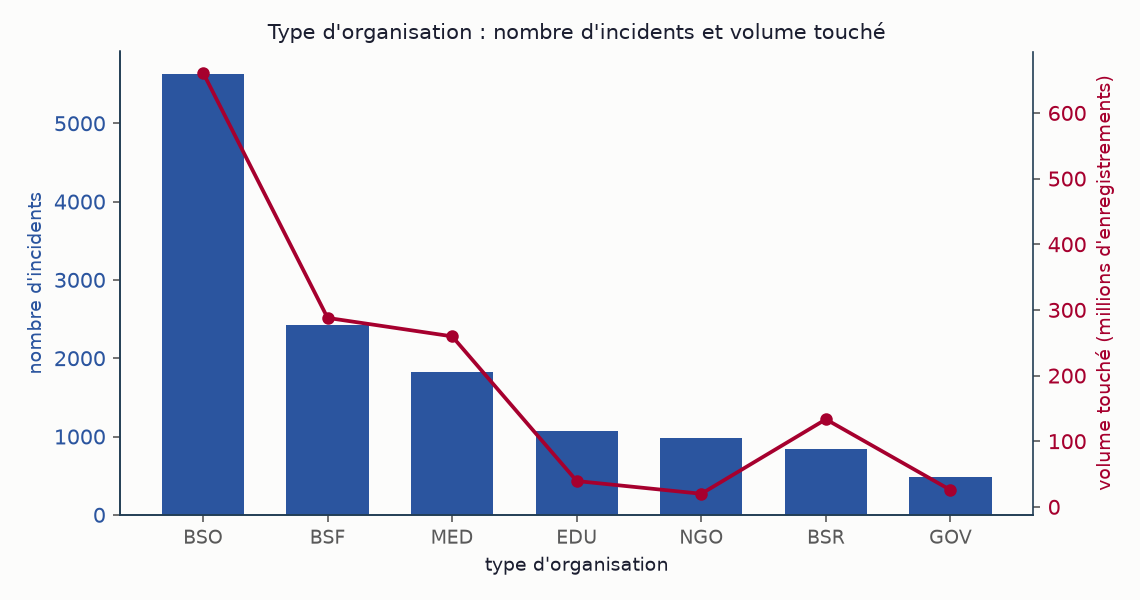
\includegraphics[width=0.88\textwidth]{D5_organisation_double_axe.png}
\caption{Nombre d'incidents (barres) et volume touché (courbe) par type d'organisation. Les deux
classements ne coïncident pas.}
% SOURCES-SCRIPTS: 104
\label{fig:organisation-double-axe}
\end{figure}

Le même décalage entre nombre et volume s'observe entre sources de notification. Une source qui ne
déclare que vingt-sept incidents en concentre plus de deux cents millions d'enregistrements : un
indicateur agrégé serait dominé par le régime déclaratif de quelques juridictions.

La figure~\ref{fig:bulles-breche} sépare ce que le seul comptage confond. Le piratage domine la fréquence,
avec $7\,430$ incidents et un impact médian de $836$ enregistrements : c'est le seul type à la fois fréquent
et lourd. La divulgation involontaire est deuxième en fréquence, mais la plus légère en
médiane, à $61$ enregistrements. À l'opposé, la fraude à la carte ne compte que quatorze incidents pour
une médiane de $860$, la plus haute du tableau. Un type rare peut donc porter une sévérité unitaire élevée
sans peser sur la charge, et l'inverse est vrai.

\begin{figure}[H]
\centering
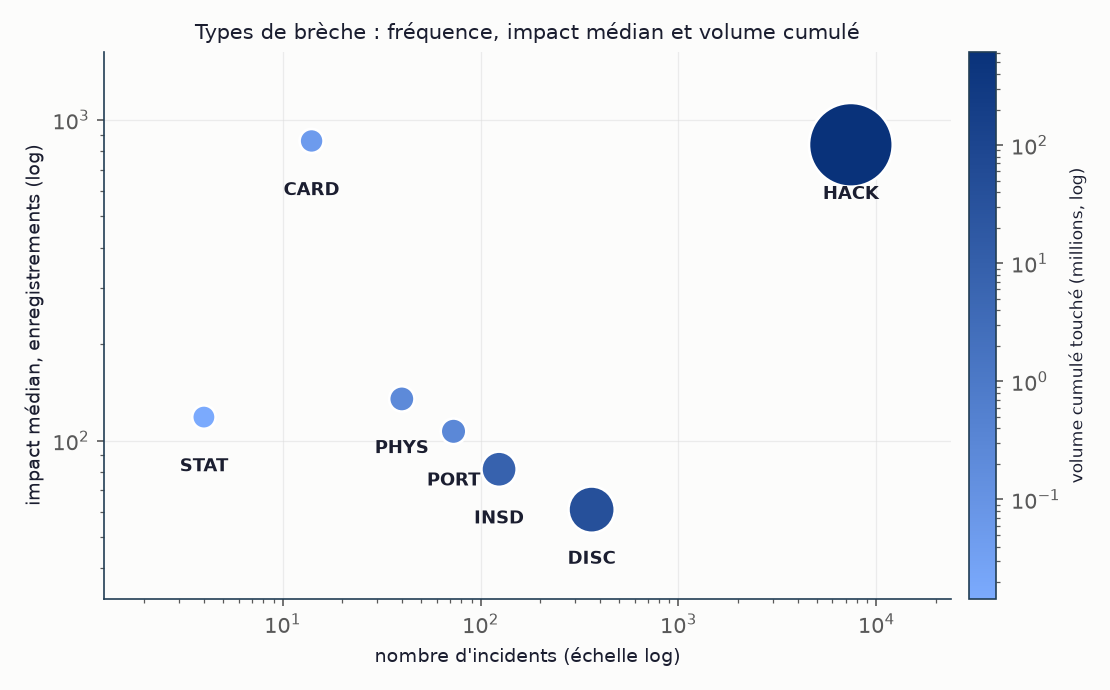
\includegraphics[width=0.74\textwidth]{D3_bulles_breche.png}
\caption{Types de brèche dans le plan fréquence contre impact médian. La taille et la teinte des disques
donnent le volume cumulé, et les deux axes sont logarithmiques.}
% SOURCES-SCRIPTS: 104
\label{fig:bulles-breche}
\end{figure}

\subsection{Association des variables qualitatives au dépassement du seuil}
\label{subsec:tests-qualitatifs}

Un actuaire qui envisage de segmenter se demande si le type d'incident ou la classe d'organisation
permettent de prédire qu'une perte dépasse un seuil élevé. Nous binarisons l'impact au troisième quartile
de chaque base, soit $8\,330$ enregistrements pour la PRC et $20{,}00$~M\$ pour SAS. Nous testons ensuite
l'indépendance par un $\chi^2$ et mesurons la force du lien par un $V$ de Cramér à correction de Bergsma.

\begin{center}\small
\renewcommand{\arraystretch}{1.15}
\begin{tabular}{@{}l l r r r@{}}
\toprule
\textbf{Base} & \textbf{Variable croisée au dépassement} & \textbf{$\chi^2$} & \textbf{ddl} &
\textbf{$V$ de Cramér} \\
\midrule
PRC & type de brèche              & $43{,}1$     & $6$  & $0{,}068$ \\
PRC & type d'organisation         & $296{,}4$    & $6$  & $0{,}148$ \\
\midrule
SAS & catégorie bâloise           & $1\,301{,}9$ & $6$  & $0{,}176$ \\
SAS & ligne métier bâloise        & $1\,238{,}5$ & $9$  & $0{,}171$ \\
SAS & secteur d'activité          & $711{,}9$    & $20$ & $0{,}128$ \\
\bottomrule
\end{tabular}
\end{center}
% SOURCES-SCRIPTS: 104

\vspace{2pt}
\noindent Les cinq tests rejettent l'indépendance, mais ce rejet n'apprend rien. Avec quinze mille et
quarante mille observations, le $\chi^2$ détecte des écarts sans portée pratique, et sa p-valeur mesure
l'effectif autant que l'association. Le renseignement est dans le $V$, une taille d'effet bornée par un
qui ne croît pas avec $n$.

Aucune des cinq associations n'atteint $0{,}20$, alors que $0{,}30$ marque
conventionnellement une association moyenne. La plus forte, la catégorie bâloise dans SAS, vaut $0{,}176$.
Ces nombres autorisent à dire que la catégorie d'un incident informe la probabilité qu'il soit lourd. Ils
n'en font pas une variable de segmentation. Segmenter par la catégorie bâloise, qui compte sept
modalités, ramènerait les $86$ excès de la calibration à une douzaine par modalité, effectif sur lequel
l'ajustement d'une queue serait très instable. C'est le premier argument en faveur d'une queue commune.

\subsection{Forme, dépendance de rang et hétérogénéité des variables quantitatives}
\label{subsec:tests-quantitatifs}
% SOURCES-SCRIPTS: 104

Nous avons chiffré la non-normalité par un test de Shapiro-Wilk, appliqué à l'échelle brute puis à
l'échelle logarithmique, sur un tirage plafonné à $5\,000$ observations à graine fixée, car la statistique
est calculable au-delà, mais sa p-valeur moins fiable. À l'échelle brute, $W$ vaut $0{,}037$ sur la PRC et $0{,}071$
sur SAS, pour une référence de un, et le rejet est total. Les moments confirment ce résultat : sur la
PRC, l'asymétrie est de $29{,}4$ et l'aplatissement de $1\,083$, contre trois pour une loi normale. Le
passage au logarithme améliore nettement la statistique sans la sauver, $W$ montant à $0{,}970$ et
$0{,}986$. La normalité est rejetée aux deux échelles. Ce test ne démontre pas une queue plus lourde
que celle d'une lognormale. Le recours à la GPD repose sur les diagnostics de dépassement de seuil
du chapitre~\ref{chap:socle}, plutôt que sur ce seul rejet global.

La corrélation de rang de Spearman mesure le lien entre le montant de perte et la taille, sur
$33\,769$ pertes à profil financier complet. Elle vaut $0{,}159$ pour le chiffre d'affaires, $0{,}139$
pour l'effectif et $0{,}068$ pour l'actif total. Ces faibles liens de rang ne suffisent pas à estimer
une élasticité en présence d'hétérogénéité. L'actif total est la moins liée des trois mesures, alors que
le bilan porte la mise à l'échelle prudentielle du chapitre~\ref{chap:resultats}.
Mesurer la taille par l'actif est donc une hypothèse du modèle, non un résultat de ces données.

Ce constat ne suppose aucune forme de loi et repose sur
un effectif plus de vingt fois supérieur à celui de la descente d'échelle. Il va dans le sens de l'élasticité de
$0{,}087$ mesurée par ailleurs, sans la confirmer au sens statistique, puisque les deux grandeurs
diffèrent. Il rend cette faible élasticité moins surprenante. Il corrobore aussi, par un chemin
indépendant, la limite d'une sévérité non plafonnée à l'échelle d'entité, inscrite au registre des
limites du chapitre~\ref{ch:robustesse}. C'est cette limite qui fait lire le besoin de capital de
l'entité notionnelle comme une extrapolation d'ordre de grandeur.

Le test de Kruskal-Wallis ne dépend pas de la normalité qui vient d'être écartée. Il rejette l'égalité
des distributions de sévérité entre classes dans les quatre configurations testées. La taille d'effet
$\varepsilon^2$ mesure l'écart : $0{,}0100$ pour le type d'organisation et $0{,}0123$ pour le type de
brèche dans la PRC, $0{,}0720$ pour la catégorie bâloise et $0{,}0785$ pour la ligne métier dans SAS. La
classe est associée à de faibles différences de rang ; ces tailles d'effet ne sont pas des parts de variance des montants.

Trois diagnostics complémentaires convergent : le $V$ de Cramér reste sous $0{,}20$, l'$\varepsilon^2$ sous
$0{,}08$ et les corrélations de rang sous $0{,}16$. La catégorie d'un incident et la taille de l'entité
qui le subit informent faiblement sa sévérité, et segmenter la queue sur l'une ou l'autre coûterait des
degrés de liberté sans pouvoir explicatif en retour. Nous ajustons donc une queue commune. Ce choix repose
sur des tailles d'effet mesurées. Il reste une hypothèse : l'indice varie selon la catégorie bâloise, et aucune
base n'observe la sévérité par pilier.


\section{Limites des données}
\label{sec:portee-donnees}

Les sources ne mesurent pas le niveau de conformité DORA d'une entité, d'où des états par pilier
posés (chapitre~\ref{chap:multietats}). Aucune base d'incidents n'est harmonisée, exhaustive et
exempte de biais de visibilité ; faute d'événements joints, la corrélation entre les pertes des
piliers ne s'estime pas, et le chapitre~\ref{chap:cascade} la remplace par une structure de
dépendance explicite. Le registre des incidents majeurs que DORA instaure atténuera ces limites sans les lever : limité aux incidents au-dessus d'un seuil de matérialité, il restera tronqué.

S'il renseigne la taille de l'entité et le prestataire en cause, il permettra de conditionner la sévérité à la taille et de cartographier les tiers (chapitre~\ref{chap:partielle}), sans changer la structure du modèle.

D'autres bases, sinistres assurantiels ou enquêtes sectorielles, auraient leurs propres biais. L'indice
de queue domine l'incertitude du modèle (chapitre~\ref{ch:robustesse}) : une base de plus ne la
réduirait que si elle apportait des pertes en montant au-delà du seuil. Les parts par vecteur tirées de
Hackmageddon sont du même ordre dans le rapport \emph{ENISA Threat Landscape 2025} \citep{enisa2025}, collecté autrement \matcomp.

Les entrées transmises au chapitre~\ref{chap:socle} sont donc la fréquence $\lambda$ et les pertes
qui servent à ajuster la queue ($\hat\xi=0{,}595$ sur OpRisk). Elles permettent de compter et de
chiffrer les incidents, sans dire quels piliers ils atteignent. Cette dernière question exige la
cascade du chapitre~\ref{chap:cascade}, puis l'examen de son identification aux
chapitres~\ref{ch:identifiabilite} et~\ref{chap:partielle}.

% SOURCES-SCRIPTS: 05 62 63 47
